\documentclass[12pt,a4paper]{article}

\usepackage[a4paper,margin=1in]{geometry}
\usepackage{graphicx}
\usepackage{booktabs}
\usepackage{amsmath,amssymb}
\usepackage{float}
\usepackage{hyperref}
\usepackage{xcolor}
\usepackage{listings}
\usepackage{enumitem}
\usepackage{fancyhdr}
\usepackage{longtable}

\hypersetup{colorlinks=true,linkcolor=blue,urlcolor=blue}

\pagestyle{fancy}
\fancyhf{}
\lhead{ICS1512}
\rhead{Machine Learning Algorithms Laboratory}
\cfoot{\thepage}

\lstset{
language=Python,
basicstyle=\ttfamily\small,
numbers=left,
frame=single,
breaklines=true,
showstringspaces=false
}

\begin{document}

\begin{tabular}{|p{4cm}|p{11cm}|}
\hline
Experiment No. & 8 \\ \hline
Experiment Title & Clustering Human Activity Recognition Data using K-Means, DBSCAN, and
Hierarchical Clustering\footnotemark\\ \hline
Student Name & Simiyon Vinscent Samuel L \\ \hline
Register Number & 3122247001062 \\ \hline
Faculty & Dr. Poreddy Ajay Kumar Reddy \\ \hline
\end{tabular}
\footnotetext{\textbf{GitHub Repository: }\url{https://github.com/blackscythe123/Machine-Learning-course}}

\section{Objective}
\begin{itemize}[nosep]
\item To cluster the UCI Human Activity Recognition (HAR) smartphone dataset with three
algorithms: K-Means, DBSCAN and Hierarchical Agglomerative Clustering (HAC).
\item To choose the number of clusters for K-Means with the elbow method and the silhouette
score, and to tune $\epsilon$ and \texttt{minPts} for DBSCAN.
\item To compare the algorithms with internal metrics (Silhouette, Davies--Bouldin,
Calinski--Harabasz) and external metrics (Adjusted Rand Index, Normalized Mutual Information)
computed against the true activity labels.
\item To visualise the clusters in two dimensions with PCA and t-SNE, and to analyse where each
algorithm agrees or disagrees with the six real activities.
\end{itemize}

\section{Problem Statement}
Each of the 10,299 samples is a 2.56-second window of smartphone accelerometer and gyroscope
readings, summarised as a 561-dimensional feature vector. The task is unsupervised: group
windows of similar movement together without being told the activity. The six activity labels
(walking, walking upstairs, walking downstairs, sitting, standing, laying) exist in the data
but are held back during fitting and used only afterwards to score the clusters. The question
the experiment asks is whether the natural structure of these sensor features matches the six
activities, and which of the three algorithms finds it best.

\section{Dataset Description}
\begin{longtable}{|p{6cm}|p{8cm}|}
\hline
Dataset Name & Human Activity Recognition Using Smartphones \\ \hline
Dataset Source & UCI Machine Learning Repository
(\url{https://archive.ics.uci.edu/dataset/240/human+activity+recognition+using+smartphones}),
the link given in the assignment \\ \hline
Number of Samples & 10,299 windows (the 7,352 training and 2,947 test windows of the original
release, pooled, since no model is trained here) \\ \hline
Number of Features & 561 time-domain and frequency-domain features (2.56 s windows of 128
readings, sampled at 50 Hz, features scaled to $[-1, 1]$ in the release) \\ \hline
Volunteers & 30, aged 19 to 48 \\ \hline
Number of Classes & 6: Walking 1722 (16.72\%), Walking Upstairs 1544 (14.99\%), Walking
Downstairs 1406 (13.65\%), Sitting 1777 (17.25\%), Standing 1906 (18.51\%), Laying 1944
(18.88\%) \\ \hline
Missing Values & 0 (verified, no imputation required) \\ \hline
Train-Test Split & None; clustering is unsupervised, so all 10,299 windows are clustered \\ \hline
\end{longtable}

\section{Exploratory Data Analysis}
\begin{figure}[H]
\centering

\includegraphics[width=\linewidth]{figures/00_eda_summary.png}
\caption{Consolidated exploratory data analysis (12 subplots, single page): (1) activity
distribution; (2--7) kernel density plots, split by activity, of the six features with the
highest ANOVA F-score against the activity label; (8) correlation heatmap of the ten
highest-scoring features; (9--11) activity-split boxplots of the three top features; (12) PCA
projection coloured by activity. Exported at 600 DPI as
\texttt{figures/00\_eda\_summary.eps} and reproduced here as PNG.}
\end{figure}

\textbf{Inference:} The six classes are reasonably balanced (1406 to 1944 windows each), so no
class dominates the clustering by size. The most discriminative features separate
\emph{static} activities from \emph{dynamic} ones rather than the six activities from each other:
the entropy features of body-acceleration jerk sit near $-1$ for sitting, standing and laying
but near $0.4$ to $0.7$ for the three walking activities, and \texttt{tGravityAcc-mean()-X}
places laying on its own around $-0.4$ while every other activity piles up near $+0.95$. The
correlation heatmap shows two blocks of near-duplicate features ($|r| \geq 0.97$ inside each
block, about $0.4$ between blocks), so the 561 features carry far fewer independent signals than
their count suggests.

\begin{figure}[H]
\centering
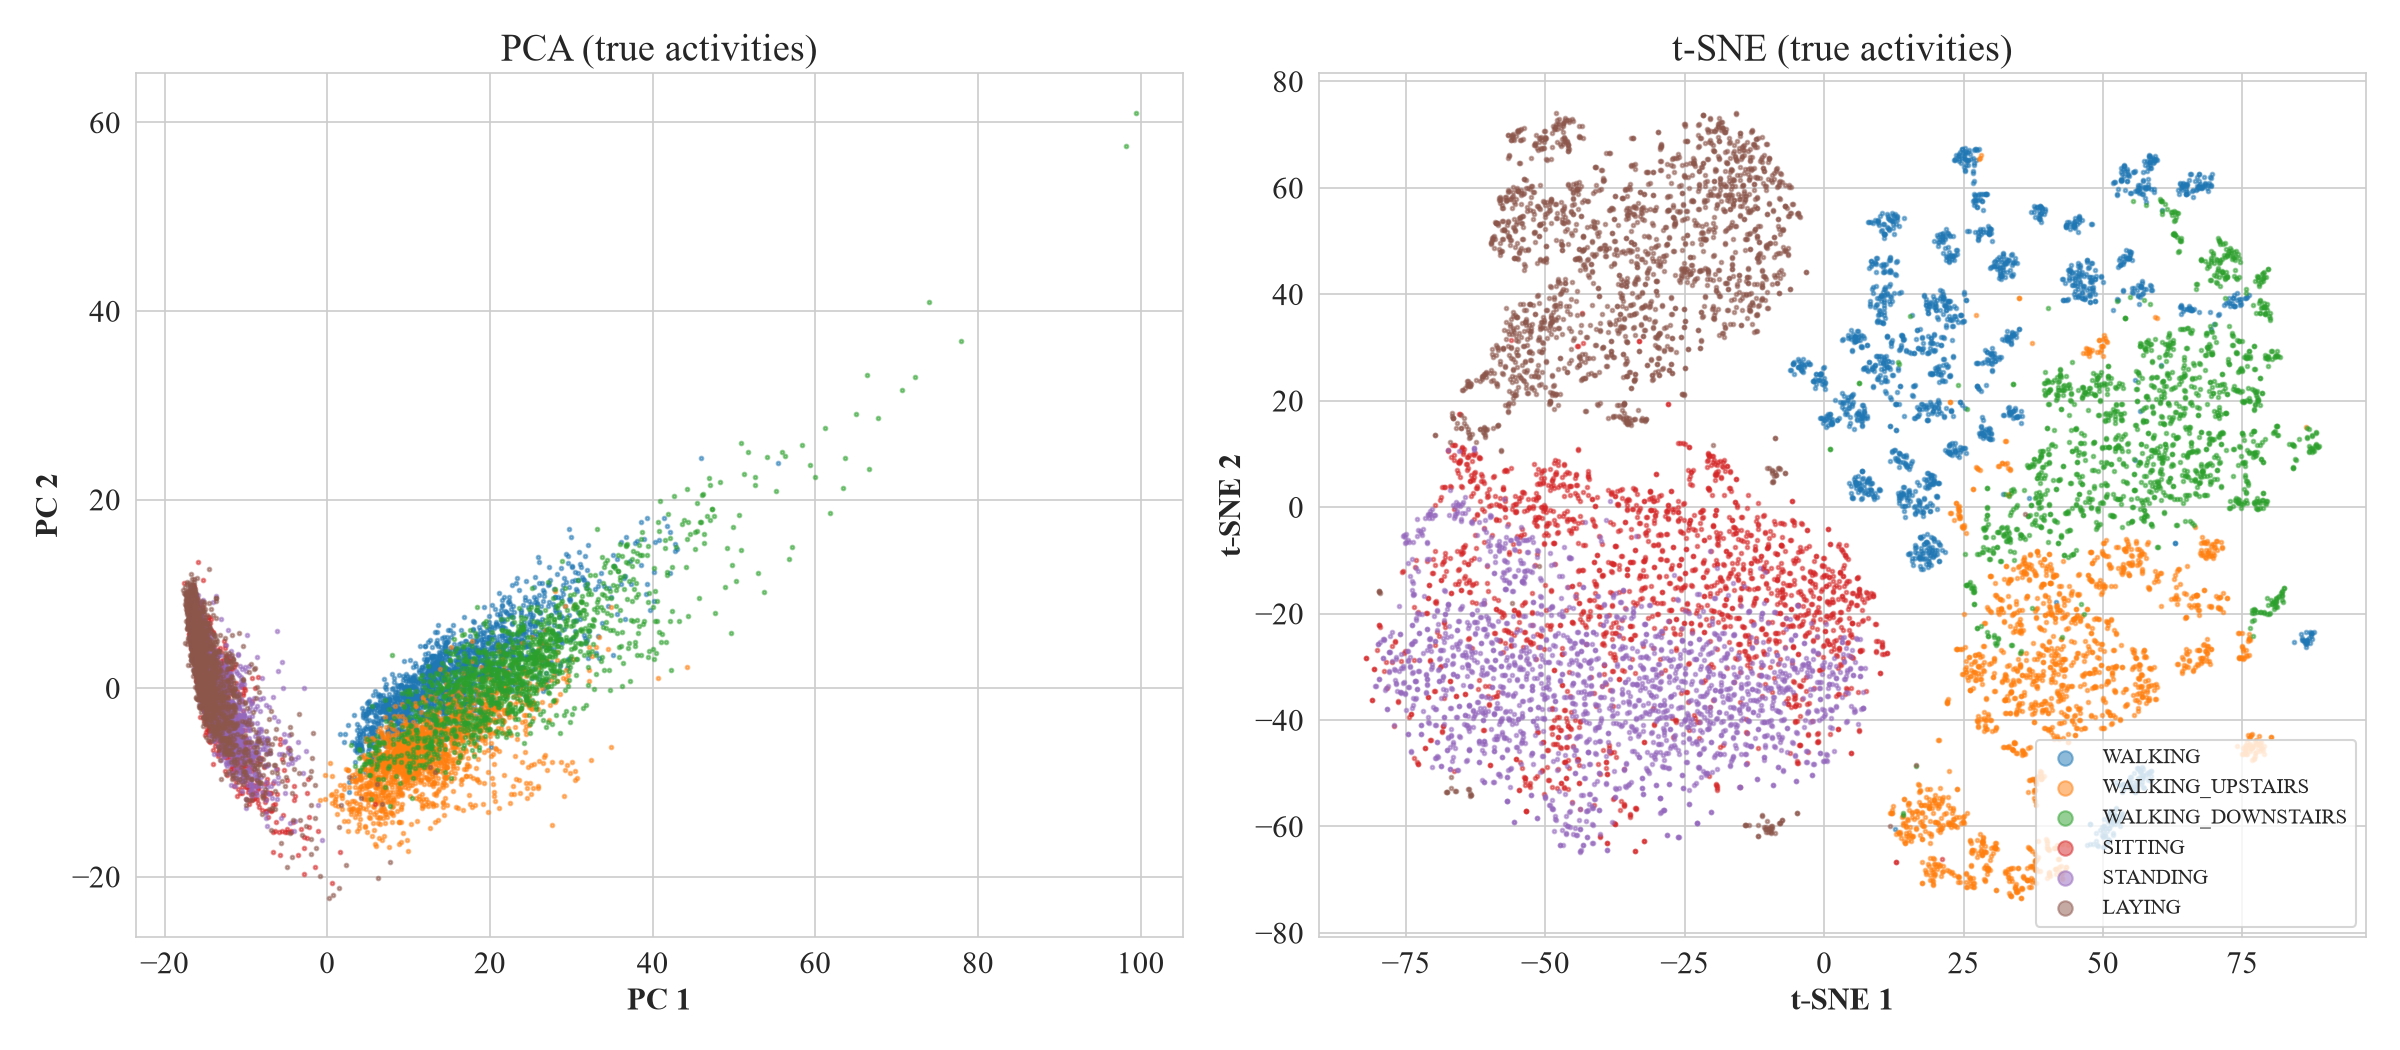
\includegraphics[width=\linewidth]{figures/01_ground_truth_pca_tsne.png}
\caption{The whole dataset projected to two dimensions with PCA (left, 56.98\% of the variance)
and t-SNE (right, run on the first 50 principal components), coloured by the true activity.}
\end{figure}
\textbf{Inference:} In the PCA view the first component alone splits the data into a tight
static group on the left and a spread-out dynamic group on the right; the two points near
$\text{PC}_1 \approx 100$ are extreme walking-downstairs windows. t-SNE shows finer structure:
laying forms its own island, sitting and standing overlap almost completely in one large mass,
and the three walking activities form neighbouring regions in which walking downstairs
overlaps both of the others. These are the overlaps any clustering algorithm has to fight
against.

\section{Data Preprocessing}
\begin{itemize}
\item \textbf{Missing values:} None found (0 missing entries in the $10299 \times 561$ matrix).
\item \textbf{Duplicate feature names:} Only 477 of the 561 feature names are unique in the raw
file (the band-energy features repeat names). A numeric suffix was added to keep column names
unique; no values were changed.
\item \textbf{Label encoding:} The activity codes 1 to 6 were mapped to their names and then
integer-encoded with \texttt{LabelEncoder}. The encoded labels are used only for colouring the
plots and for ARI and NMI, never for fitting.
\item \textbf{Feature scaling:} \texttt{StandardScaler} applied to all 561 features. K-Means, Ward
linkage and DBSCAN all rely on Euclidean distance, so scaling makes every feature contribute
equally to that distance.
\item \textbf{Dimensionality reduction:} PCA to 2 components (56.98\% of variance) for the
scatter plots, and PCA to 50 components (87.10\% of variance) as the input to t-SNE and as a
second, lower-dimensional space for DBSCAN. t-SNE used perplexity 30, PCA initialisation and
\texttt{random\_state=42}.
\item \textbf{Train-test split:} Not applicable, since no supervised model is trained.
\end{itemize}

\section{Machine Learning Algorithm}

\subsection*{K-Means}
K-Means partitions the data into $k$ clusters by minimising the within-cluster sum of squares
(WCSS), $\sum_{j=1}^{k}\sum_{x \in C_j}\lVert x - \mu_j \rVert^2$. It starts from $k$ centroids,
assigns each point to its nearest centroid, recomputes each centroid as the mean of its points,
and repeats until the assignments stop changing. It assumes compact, roughly spherical clusters
of similar size. The number of clusters $k$ must be chosen in advance; here it is chosen with the
elbow method (the point where the drop in WCSS levels off) and the silhouette score.

\subsection*{DBSCAN}
DBSCAN labels a point as a \emph{core} point if at least \texttt{minPts} points (itself
included) lie within distance $\epsilon$, joins core points that are within $\epsilon$ of each
other into clusters, attaches \emph{border} points to a nearby core point, and marks everything
else as \emph{noise}. It needs no cluster count, can find clusters of arbitrary shape and flags
outliers, but a single global $\epsilon$ struggles when clusters have different densities. A
$k$-distance plot (each point's distance to its $k$-th nearest neighbour, sorted) is the usual
guide for choosing $\epsilon$.

\subsection*{Hierarchical Agglomerative Clustering}
HAC starts with every point as its own cluster and repeatedly merges the two closest clusters,
recording the merge heights in a dendrogram; cutting the dendrogram at a chosen height or cluster
count gives a flat clustering. The linkage rule defines cluster-to-cluster distance:
\textbf{single} (closest pair of points), \textbf{complete} (farthest pair), \textbf{average}
(mean over all pairs) or \textbf{Ward} (the merge that increases total within-cluster variance
the least, the same objective K-Means minimises).

\subsection*{Evaluation Metrics}
\begin{itemize}
\item \textbf{Silhouette} $s = (b - a)/\max(a, b)$, where $a$ is a point's mean distance to its
own cluster and $b$ its mean distance to the nearest other cluster; range $[-1, 1]$, higher is
better.
\item \textbf{Davies--Bouldin} index: the average, over clusters, of the worst ratio of
within-cluster spread to between-cluster separation; lower is better.
\item \textbf{Calinski--Harabasz} index: the ratio of between-cluster to within-cluster
dispersion, adjusted for the number of clusters; higher is better.
\item \textbf{Adjusted Rand Index (ARI)}: pair-counting agreement with the true labels, corrected
for chance ($0$ is chance level, $1$ is perfect).
\item \textbf{Normalized Mutual Information (NMI)}: shared information between the clustering
and the true labels, scaled to $[0, 1]$.
\end{itemize}
DBSCAN noise points have no cluster, so the three internal metrics are computed on the non-noise
points only, while ARI and NMI treat noise as one extra label.

\section{Experimental Setup}
\begin{tabular}{ll}
\toprule
Python Version & 3.13.14 \\
Scikit-Learn Version & 1.9.0 \\
SciPy Version & 1.18.0 \\
IDE & Jupyter Notebook \\
Operating System & Windows 11 \\
Hardware & Intel Core Ultra 9 (CPU only; the GPU was not needed) \\
\bottomrule
\end{tabular}

\section{Parameter Selection}
No label was used to choose any parameter below; ARI and NMI were computed afterwards.

\begin{longtable}{p{3.2cm}p{11.8cm}}
\toprule
Algorithm & Search and selection rule \\
\midrule
K-Means & $k \in \{2, \dots, 8\}$, \texttt{n\_init=10}, \texttt{random\_state=42}. The elbow $k$ is
the point of the WCSS curve farthest from the straight line joining its two end points; the
silhouette $k$ is the one with the highest silhouette score. When the two disagree, the
silhouette score decides, and $k=6$ (the true number of activities) is also reported. \\
DBSCAN & Candidate $\epsilon$ values are the 20th, 35th, 50th, 65th, 80th and 90th percentiles of
the sorted 10th-nearest-neighbour distances (Figure~\ref{fig:kdist}), crossed with
$\texttt{minPts} \in \{5, 10, 20\}$, giving 18 settings per space. Two spaces were searched: the
full 561-D standardized space and the 50-component PCA space. A setting is eligible if it finds
2 to 12 clusters with at most 30\% noise; among eligible settings the highest silhouette wins. \\
HAC & Euclidean distance with single, complete, average and Ward linkage, each cut at 6
clusters. Ward is the required method; the other three are compared to it. The Ward result from
\texttt{scikit-learn}'s \texttt{AgglomerativeClustering} agrees exactly with SciPy's
(ARI $= 1.0$). \\
\bottomrule
\end{longtable}

\section{Results}

\subsection*{Table 1: K-Means Elbow Method Results}
\begin{longtable}{ccccccc}
\toprule
$k$ & WCSS ($\times 10^6$) & Silhouette & Davies--Bouldin & Calinski--Harabasz & ARI & NMI \\
\midrule
\textbf{2} & \textbf{3.2729} & \textbf{0.3937} & \textbf{1.0707} & \textbf{7880.8} & \textbf{0.3296} & \textbf{0.5455} \\
3 & 2.9211 & 0.3155 & 1.7865 & 5034.5 & 0.3317 & 0.5183 \\
4 & 2.7816 & 0.1500 & 2.3422 & 3696.3 & 0.2990 & 0.4694 \\
5 & 2.6548 & 0.1286 & 2.4108 & 3027.3 & 0.2912 & 0.4607 \\
6 & 2.5772 & 0.1099 & 2.3836 & 2556.5 & 0.4196 & 0.5593 \\
7 & 2.5198 & 0.0816 & 2.6752 & 2217.9 & 0.4332 & 0.5546 \\
8 & 2.4654 & 0.0749 & 2.6106 & 1975.2 & 0.4266 & 0.5516 \\
\bottomrule
\end{longtable}

\textbf{Inference:} WCSS falls smoothly and never bends sharply: successive drops are 10.8\%,
4.8\%, 4.6\%, 2.9\%, 2.2\% and 2.2\% as $k$ goes from 2 up to 8. The chord rule places the elbow at
$k=4$, but the curve is close to a straight line beyond $k=3$, so the elbow is a weak signal. The
silhouette score is much clearer: it is highest at $k=2$ (0.3937), falls to 0.3155 at $k=3$, and
collapses to 0.1500 at $k=4$ and below. \textbf{Selected $k = 2$}, because it has the highest
silhouette, the highest Calinski--Harabasz score and the lowest Davies--Bouldin index of the seven
values, and because it corresponds to a real physical split (static versus dynamic activity, see
Discussion). The elbow and silhouette rules disagree (4 versus 2), which is why the six-cluster
model is reported next to it throughout.

\subsection*{DBSCAN Parameter Grids}
Selected settings are in bold. Noise is the share of windows labelled $-1$; ``--'' means the
metric is undefined because at most one cluster was found.

\begin{longtable}{ccccccccc}
\multicolumn{9}{l}{\textbf{Full 561-D standardized space}} \\
\toprule
$\epsilon$ & minPts & Clusters & Noise (\%) & Sil. & DB & CH & ARI & NMI \\
\midrule
10.76 & 5 & 35 & 60.7 & -0.0101 & 1.6878 & 54.9 & 0.1166 & 0.2644 \\
10.76 & 10 & 12 & 65.6 & 0.0797 & 1.4944 & 79.6 & 0.0974 & 0.2332 \\
10.76 & 20 & 3 & 69.9 & 0.1242 & 1.3356 & 122.0 & 0.0791 & 0.2040 \\
11.82 & 5 & 32 & 47.1 & 0.0612 & 1.9479 & 125.4 & 0.1940 & 0.3635 \\
11.82 & 10 & 20 & 52.1 & 0.0752 & 2.0926 & 131.7 & 0.1793 & 0.3355 \\
11.82 & 20 & 10 & 57.2 & 0.1383 & 1.7132 & 133.3 & 0.1650 & 0.3060 \\
13.15 & 5 & 30 & 33.2 & 0.3006 & 1.6967 & 209.5 & 0.2602 & 0.4073 \\
13.15 & 10 & 14 & 37.6 & 0.0634 & 2.0182 & 359.5 & 0.2490 & 0.3977 \\
13.15 & 20 & 4 & 42.6 & 0.3557 & 1.7679 & 1116.2 & 0.2371 & 0.3842 \\
14.72 & 5 & 22 & 21.2 & 0.1252 & 1.4010 & 29.4 & 0.0737 & 0.1576 \\
14.72 & 10 & 5 & 24.7 & 0.2325 & 1.0442 & 45.0 & 0.0847 & 0.1565 \\
14.72 & 20 & 2 & 28.4 & 0.2258 & 1.0469 & 41.0 & 0.0998 & 0.1702 \\
17.07 & 5 & 5 & 9.8 & 0.0993 & 1.0893 & 41.0 & 0.0239 & 0.0820 \\
\textbf{17.07} & \textbf{10} & \textbf{2} & \textbf{11.5} & \textbf{0.3396} & \textbf{0.8729} & \textbf{103.2} & \textbf{0.0298} & \textbf{0.0882} \\
17.07 & 20 & 3 & 14.3 & 0.2809 & 0.9274 & 94.8 & 0.0415 & 0.1111 \\
19.45 & 5 & 2 & 4.8 & 0.2951 & 0.9125 & 11.7 & 0.0083 & 0.0407 \\
19.45 & 10 & 1 & 5.5 & -- & -- & -- & 0.0100 & 0.0452 \\
19.45 & 20 & 1 & 6.3 & -- & -- & -- & 0.0116 & 0.0480 \\
\bottomrule
\end{longtable}

\begin{longtable}{ccccccccc}
\multicolumn{9}{l}{\textbf{50-component PCA space}} \\
\toprule
$\epsilon$ & minPts & Clusters & Noise (\%) & Sil. & DB & CH & ARI & NMI \\
\midrule
7.13 & 5 & 21 & 63.4 & 0.0140 & 1.4454 & 38.9 & 0.1154 & 0.2506 \\
7.13 & 10 & 6 & 67.2 & 0.0999 & 1.2795 & 53.9 & 0.0948 & 0.2217 \\
7.13 & 20 & 1 & 71.3 & -- & -- & -- & 0.0753 & 0.1940 \\
8.18 & 5 & 36 & 49.2 & 0.1617 & 1.8896 & 80.6 & 0.2016 & 0.3561 \\
8.18 & 10 & 12 & 54.0 & 0.3663 & 1.7603 & 119.2 & 0.1914 & 0.3333 \\
8.18 & 20 & 4 & 58.0 & 0.1241 & 1.4405 & 114.7 & 0.1756 & 0.3092 \\
9.55 & 5 & 40 & 32.0 & 0.2770 & 1.7189 & 160.1 & 0.2718 & 0.4221 \\
9.55 & 10 & 10 & 38.0 & 0.3297 & 1.7628 & 470.5 & 0.2602 & 0.4126 \\
9.55 & 20 & 4 & 44.0 & 0.3447 & 1.8133 & 868.6 & 0.2502 & 0.4036 \\
10.98 & 5 & 18 & 19.0 & 0.2830 & 1.5581 & 452.7 & 0.3217 & 0.4740 \\
10.98 & 10 & 12 & 22.8 & 0.3095 & 1.9324 & 616.8 & 0.3190 & 0.4705 \\
10.98 & 20 & 5 & 27.9 & 0.3226 & 1.6488 & 1393.2 & 0.3037 & 0.4575 \\
12.76 & 5 & 7 & 8.4 & 0.0656 & 1.1214 & 36.5 & 0.0207 & 0.0793 \\
12.76 & 10 & 4 & 10.7 & 0.2606 & 0.9453 & 60.4 & 0.0277 & 0.0877 \\
12.76 & 20 & 3 & 14.6 & 0.2793 & 0.9205 & 92.2 & 0.0438 & 0.1159 \\
14.68 & 5 & 4 & 3.9 & 0.2569 & 0.9991 & 22.4 & 0.0062 & 0.0336 \\
14.68 & 10 & 3 & 5.1 & 0.3108 & 0.9298 & 103.0 & 0.0099 & 0.0525 \\
\textbf{14.68} & \textbf{20} & \textbf{2} & \textbf{6.3} & \textbf{0.3271} & \textbf{0.9138} & \textbf{120.7} & \textbf{0.0119} & \textbf{0.0540} \\
\bottomrule
\end{longtable}

\textbf{Inference:} Both grids show the same trade-off. Settings that find 10 or more clusters
(up to 35 in the full space and 40 in the PCA space) label 19\% to 66\% of the windows as noise,
while the largest $\epsilon$ values leave only 4\% to 15\% noise but merge everything into a
handful of clusters: no setting with under 15\% noise finds more than 5 clusters in the full
space or more than 7 in the PCA space. The eligibility rule therefore selected a near-trivial
solution in both spaces: two
clusters and 11.5\% noise at $\epsilon=17.07$, $\texttt{minPts}=10$ (full space), and two clusters
and 6.3\% noise at $\epsilon=14.68$, $\texttt{minPts}=20$ (PCA space). For the full-space choice
the two clusters contain 9079 and 31 windows, with 1189 noise windows. The settings with the
highest ARI (0.2602 in the full space, 0.3217 in the PCA space) break the eligibility rule
(30 clusters at 33\% noise, and 18 clusters at 19\% noise) and are still below K-Means and Ward
at six clusters.

\subsection*{Hierarchical Clustering: Linkage Comparison (cut at 6 clusters)}
\begin{longtable}{lccccccc}
\toprule
Linkage & Cophenetic & Largest cluster (\%) & Sil. & DB & CH & ARI & NMI \\
\midrule
Single & 0.8139 & 99.9 & 0.5601 & 0.2733 & 28.9 & 0.0001 & 0.0013 \\
Complete & 0.7523 & 54.6 & 0.3792 & 1.3004 & 1898.4 & 0.3294 & 0.5421 \\
Average & 0.8557 & 98.5 & 0.4431 & 1.1020 & 161.1 & 0.0024 & 0.0220 \\
\textbf{Ward} & \textbf{0.6767} & \textbf{31.1} & \textbf{0.1170} & \textbf{2.4820} & \textbf{2349.7} & \textbf{0.4599} & \textbf{0.6015} \\
\bottomrule
\end{longtable}

\textbf{Inference:} Linkage changes the outcome completely. Single linkage puts 99.9\% of the
windows in one cluster and average linkage 98.5\%, so both are effectively ``one giant cluster
plus a few outlier windows'' (ARI close to 0). Complete linkage gives a more balanced split
(largest cluster 54.6\%, ARI 0.3294), and Ward gives the most balanced one (largest cluster
31.1\%) with the best agreement with the true activities (ARI 0.4599, NMI 0.6015). The
cophenetic correlation ranks the linkages in almost the opposite order (Ward lowest at 0.6767,
average highest at 0.8557), so here it measures how well the tree preserves distances, not how
useful the clusters are.

\subsection*{Algorithm Comparison}
\begin{longtable}{lccccccc}
\toprule
Model & Clusters & Noise (\%) & Sil. & DB & CH & ARI & NMI \\
\midrule
K-Means ($k=2$) & 2 & 0.0 & \textbf{0.3937} & 1.0707 & \textbf{7880.8} & 0.3296 & 0.5455 \\
K-Means ($k=6$) & 6 & 0.0 & 0.1099 & 2.3836 & 2556.5 & 0.4196 & 0.5593 \\
DBSCAN (561-D) & 2 & 11.5 & 0.3396 & \textbf{0.8729} & 103.2 & 0.0298 & 0.0882 \\
DBSCAN (PCA-50) & 2 & 6.3 & 0.3271 & 0.9138 & 120.7 & 0.0119 & 0.0540 \\
HAC Ward ($k=6$) & 6 & 0.0 & 0.1170 & 2.4820 & 2349.7 & \textbf{0.4599} & \textbf{0.6015} \\
\bottomrule
\end{longtable}

\textbf{Inference:} No model wins every column. K-Means with $k=2$ has the best silhouette and
Calinski--Harabasz score, DBSCAN has the best Davies--Bouldin index, and Ward has the best ARI
and NMI. The internal metrics favour the fewest clusters, while the external metrics favour the
six-cluster models, which is the central tension of this experiment.

\section{Result Visualization}

\begin{figure}[H]
\centering
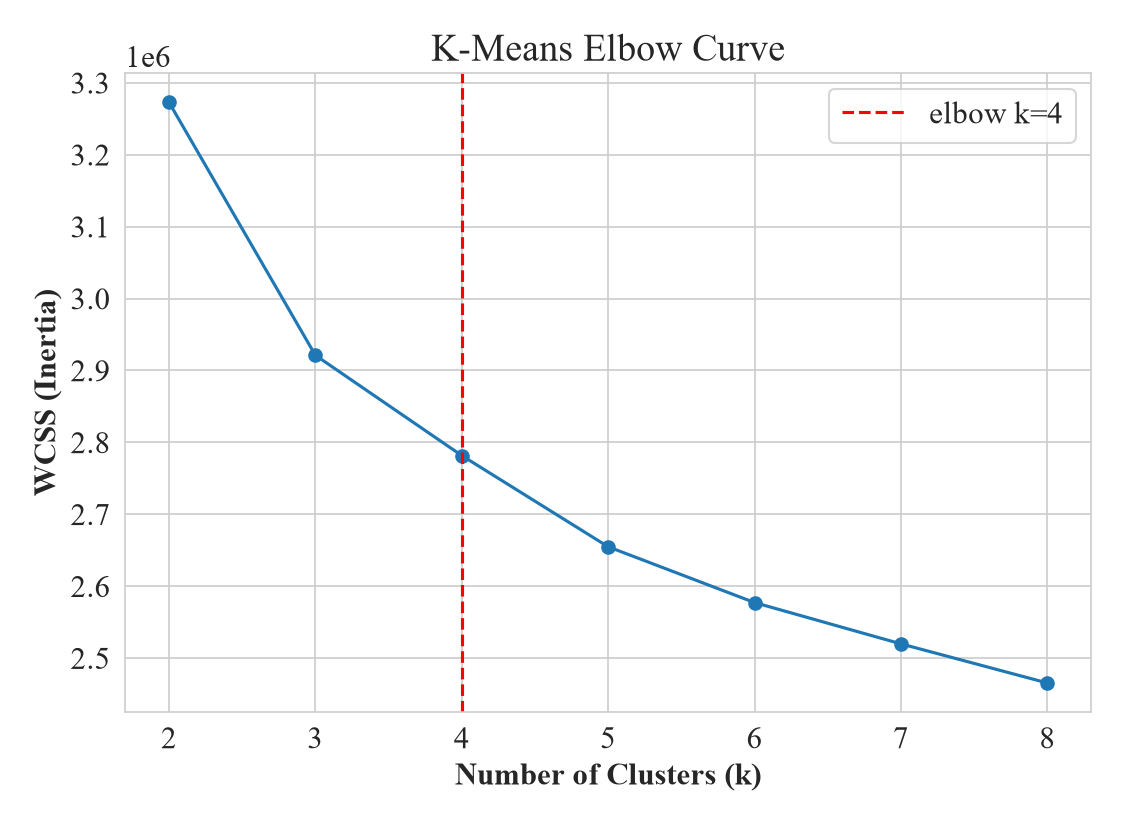
\includegraphics[width=0.48\linewidth]{figures/02_kmeans_elbow.png}\hfill
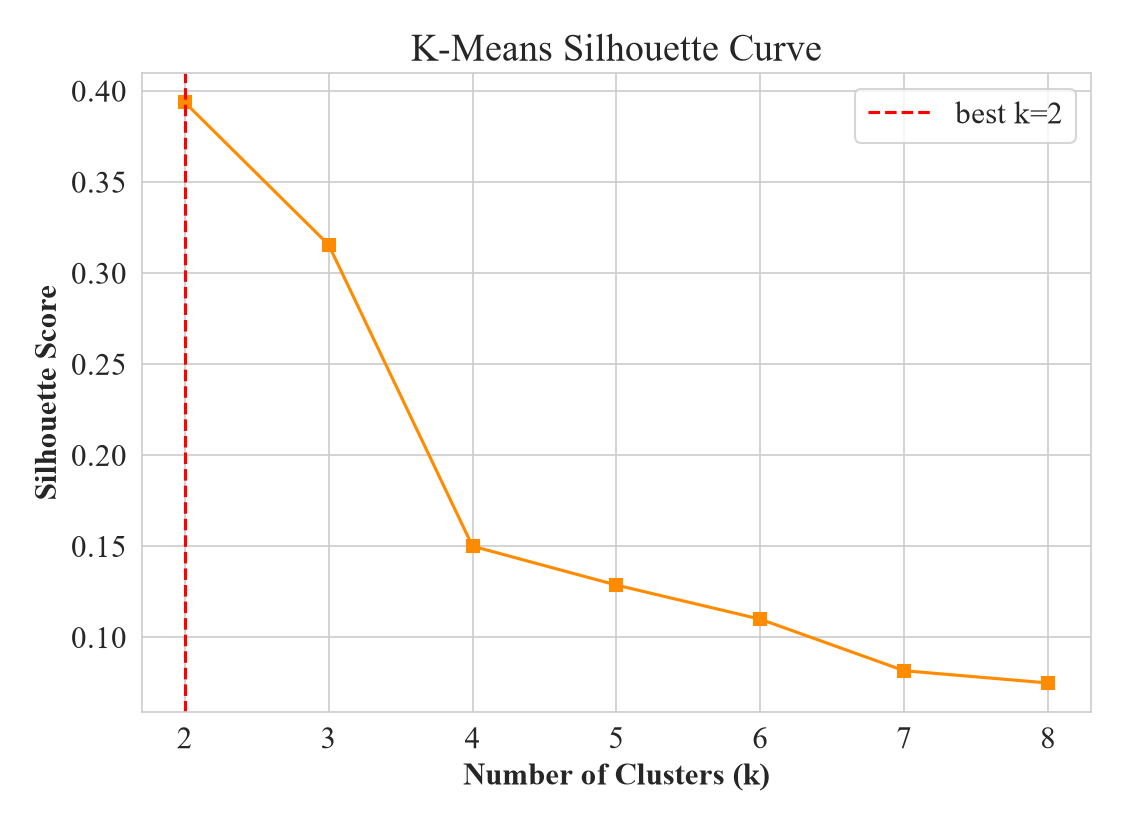
\includegraphics[width=0.48\linewidth]{figures/03_kmeans_silhouette.png}
\caption{K-Means elbow curve (left, WCSS against $k$, with the chord-based elbow at $k=4$
marked) and silhouette curve (right, with the best $k=2$ marked).}
\end{figure}
\textbf{Inference:} The elbow curve is nearly straight after $k=3$, so its ``elbow'' is a matter
of judgement, whereas the silhouette curve has an unambiguous peak at $k=2$ followed by a sharp
drop between $k=3$ and $k=4$.

\begin{figure}[H]
\centering
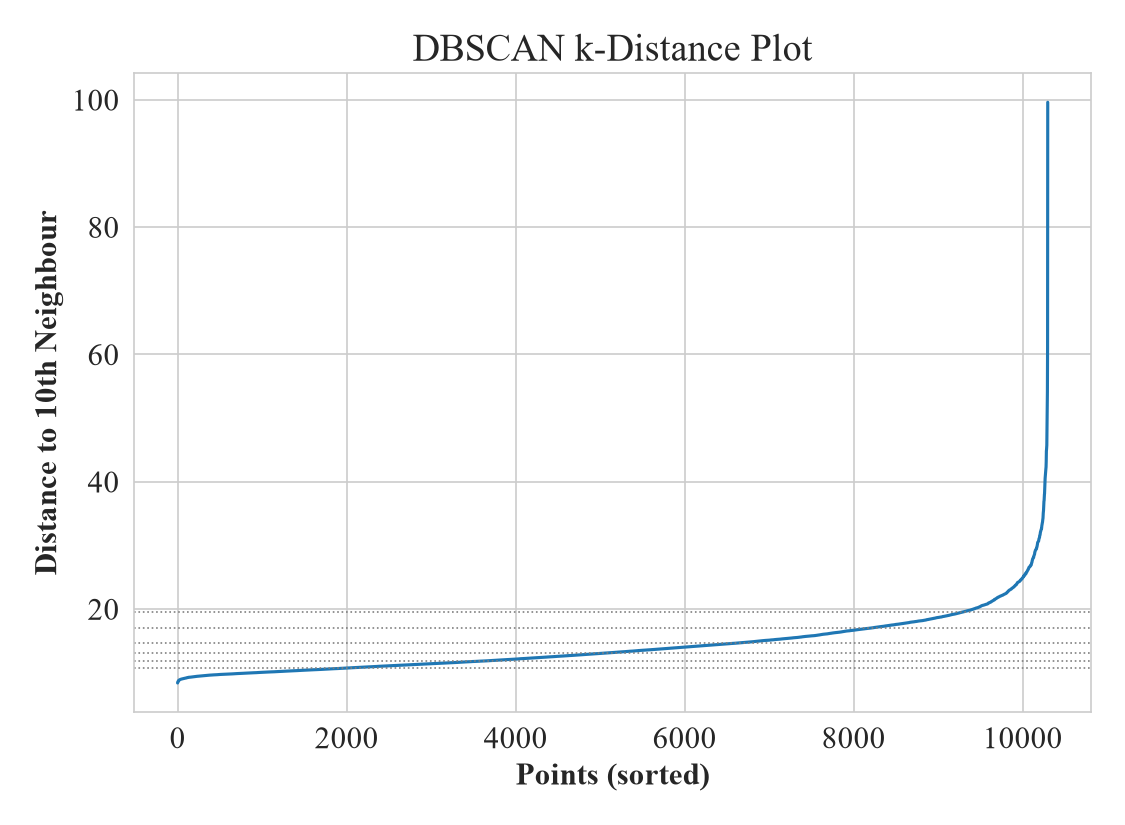
\includegraphics[width=0.6\linewidth]{figures/04_dbscan_kdistance.png}
\caption{Sorted distance to the 10th nearest neighbour for all windows in the full standardized
space. The dotted horizontal lines are the six candidate $\epsilon$ values.}
\label{fig:kdist}
\end{figure}
\textbf{Inference:} The curve rises gently from about 9 to about 20 across 90\% of the points and
then shoots up for the last few percent, so there is no single knee. That explains why the
$\epsilon$ grid trades noise against cluster count instead of finding a clean threshold: a small
group of windows (up to a distance near 100) is very far from everything else.

\begin{figure}[H]
\centering
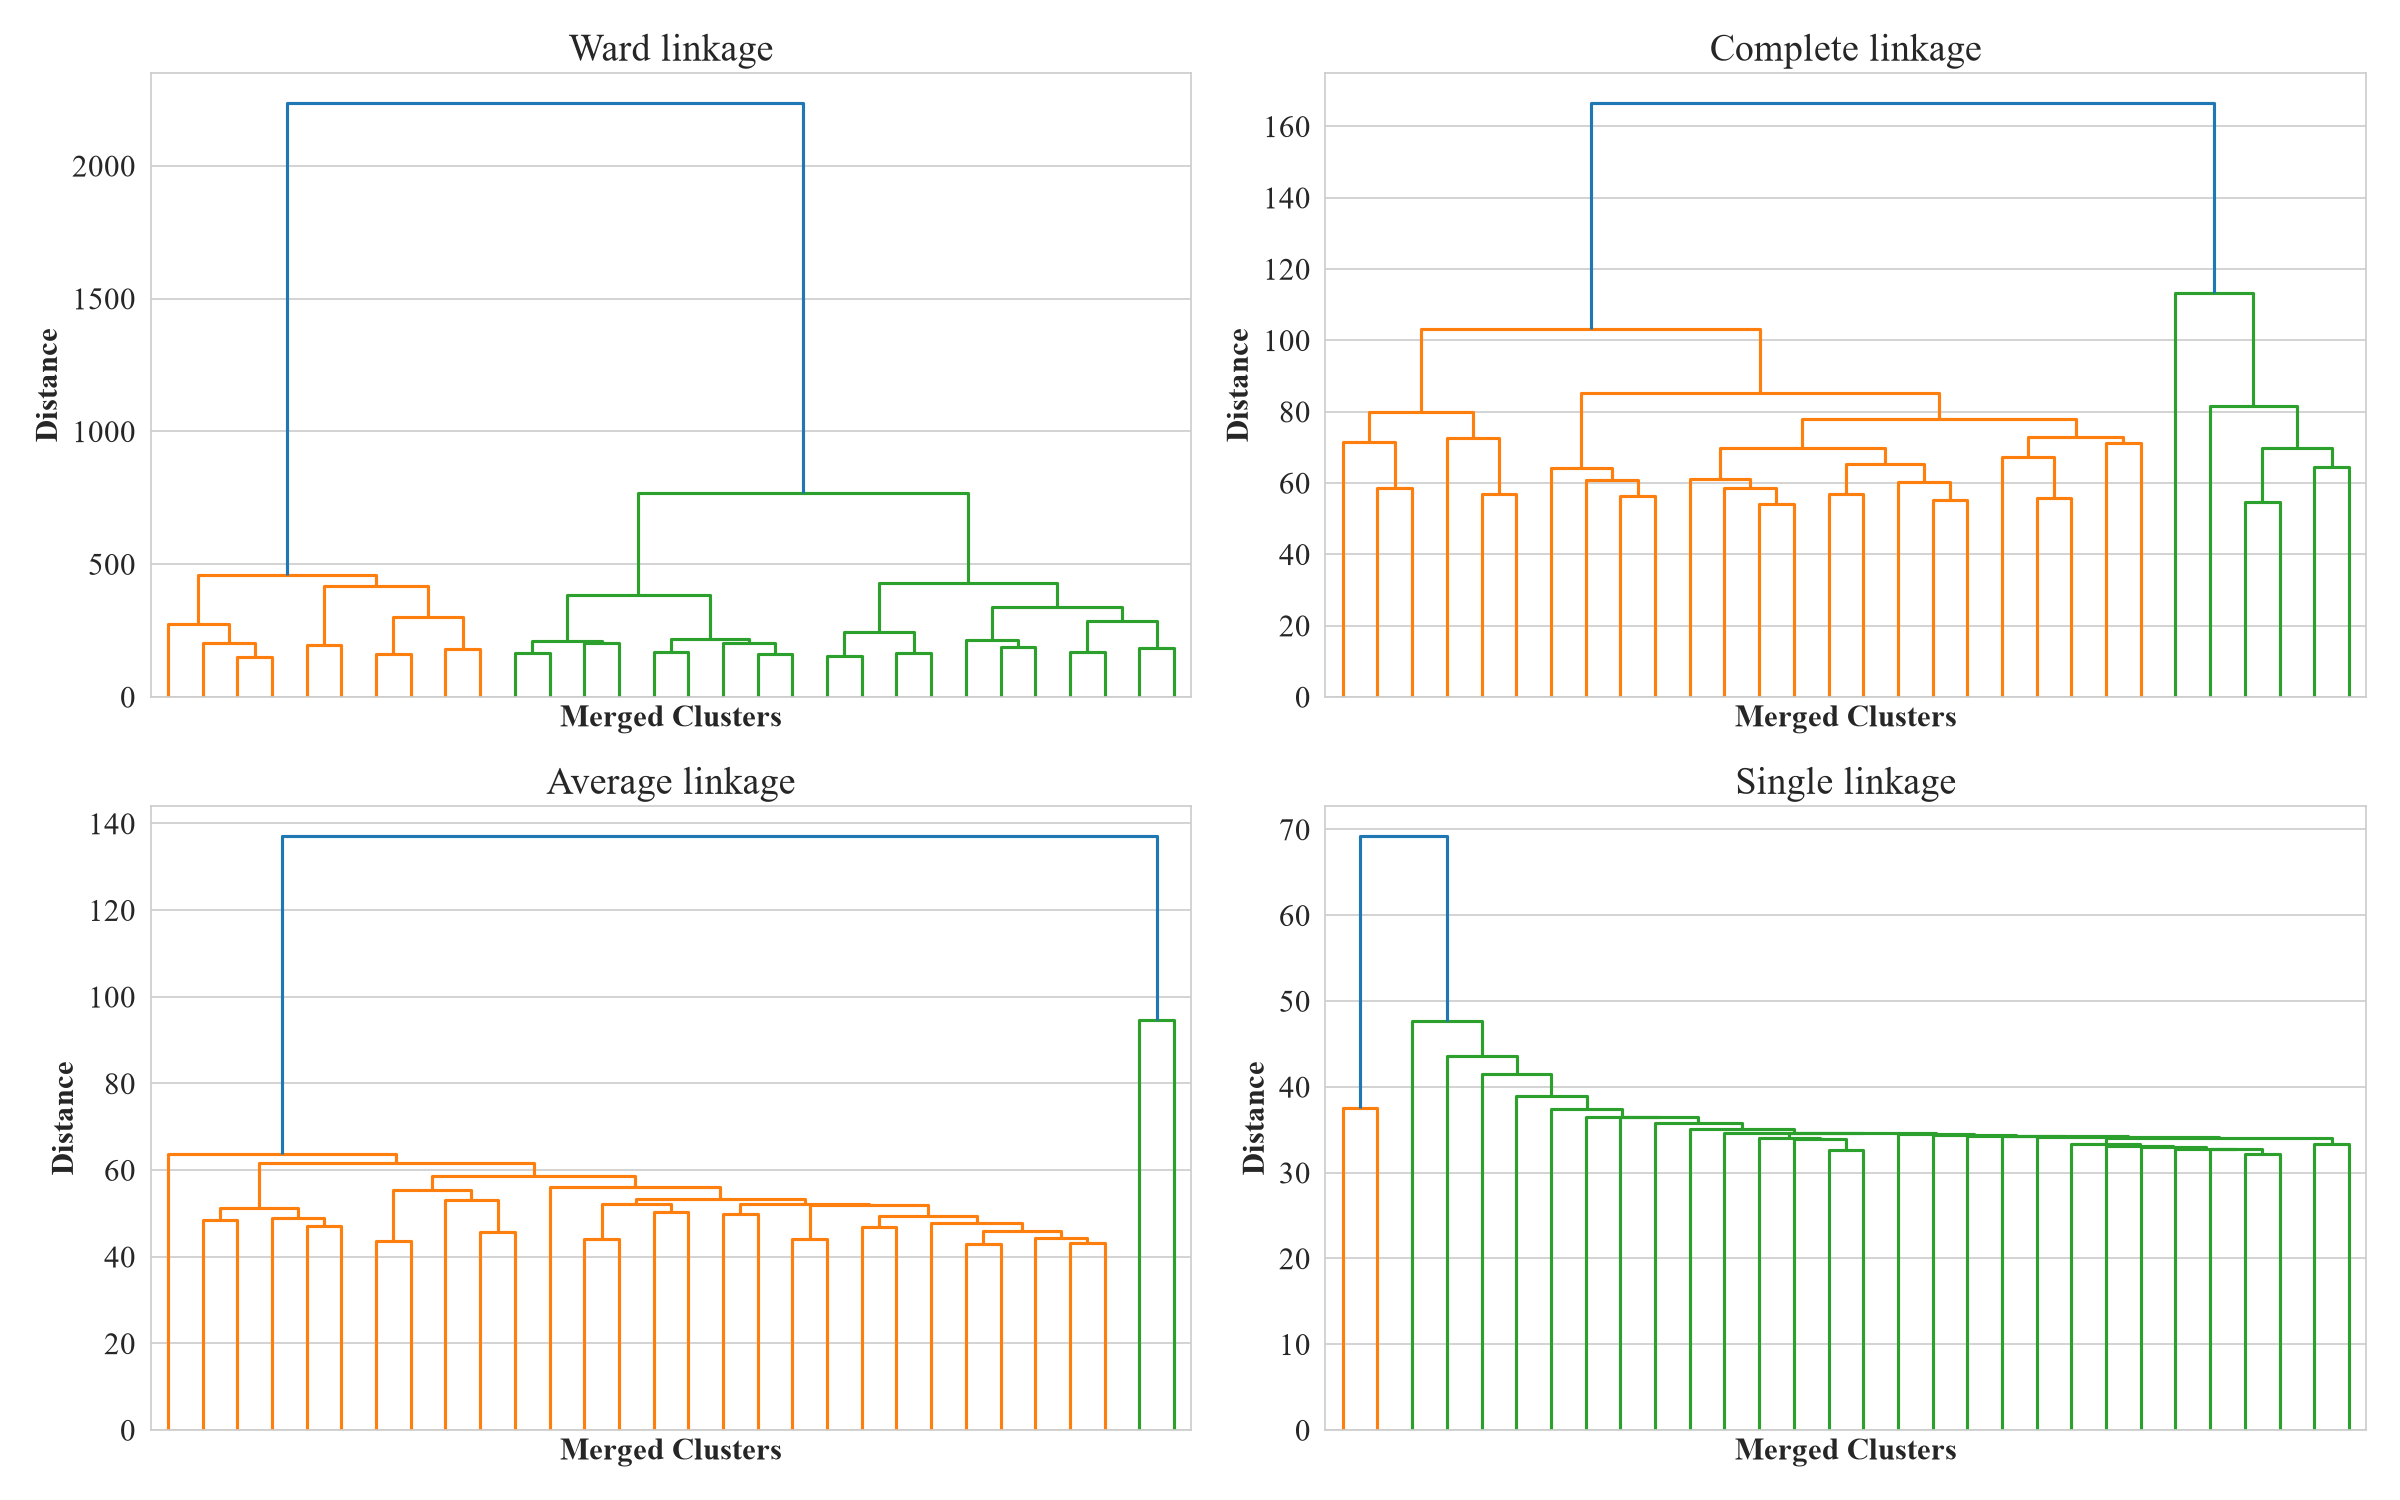
\includegraphics[width=\linewidth]{figures/05_dendrograms.png}
\caption{Dendrograms (last 30 merges shown) for Ward, complete, average and single linkage.}
\end{figure}
\textbf{Inference:} The Ward dendrogram has a very clear top-level split at a height of 2236.6,
about three times the next merge (768.7). Cutting Ward's tree into just two clusters gives
exactly the static versus dynamic separation: all 5627 sitting, standing and laying windows in
one cluster and all 4672 walking windows in the other, with no window misplaced. Complete linkage also splits into two main branches. Average linkage separates
one small branch from a large one, and single linkage forms the long chain typical of the method,
peeling off one small group at the very top.

\begin{figure}[H]
\centering
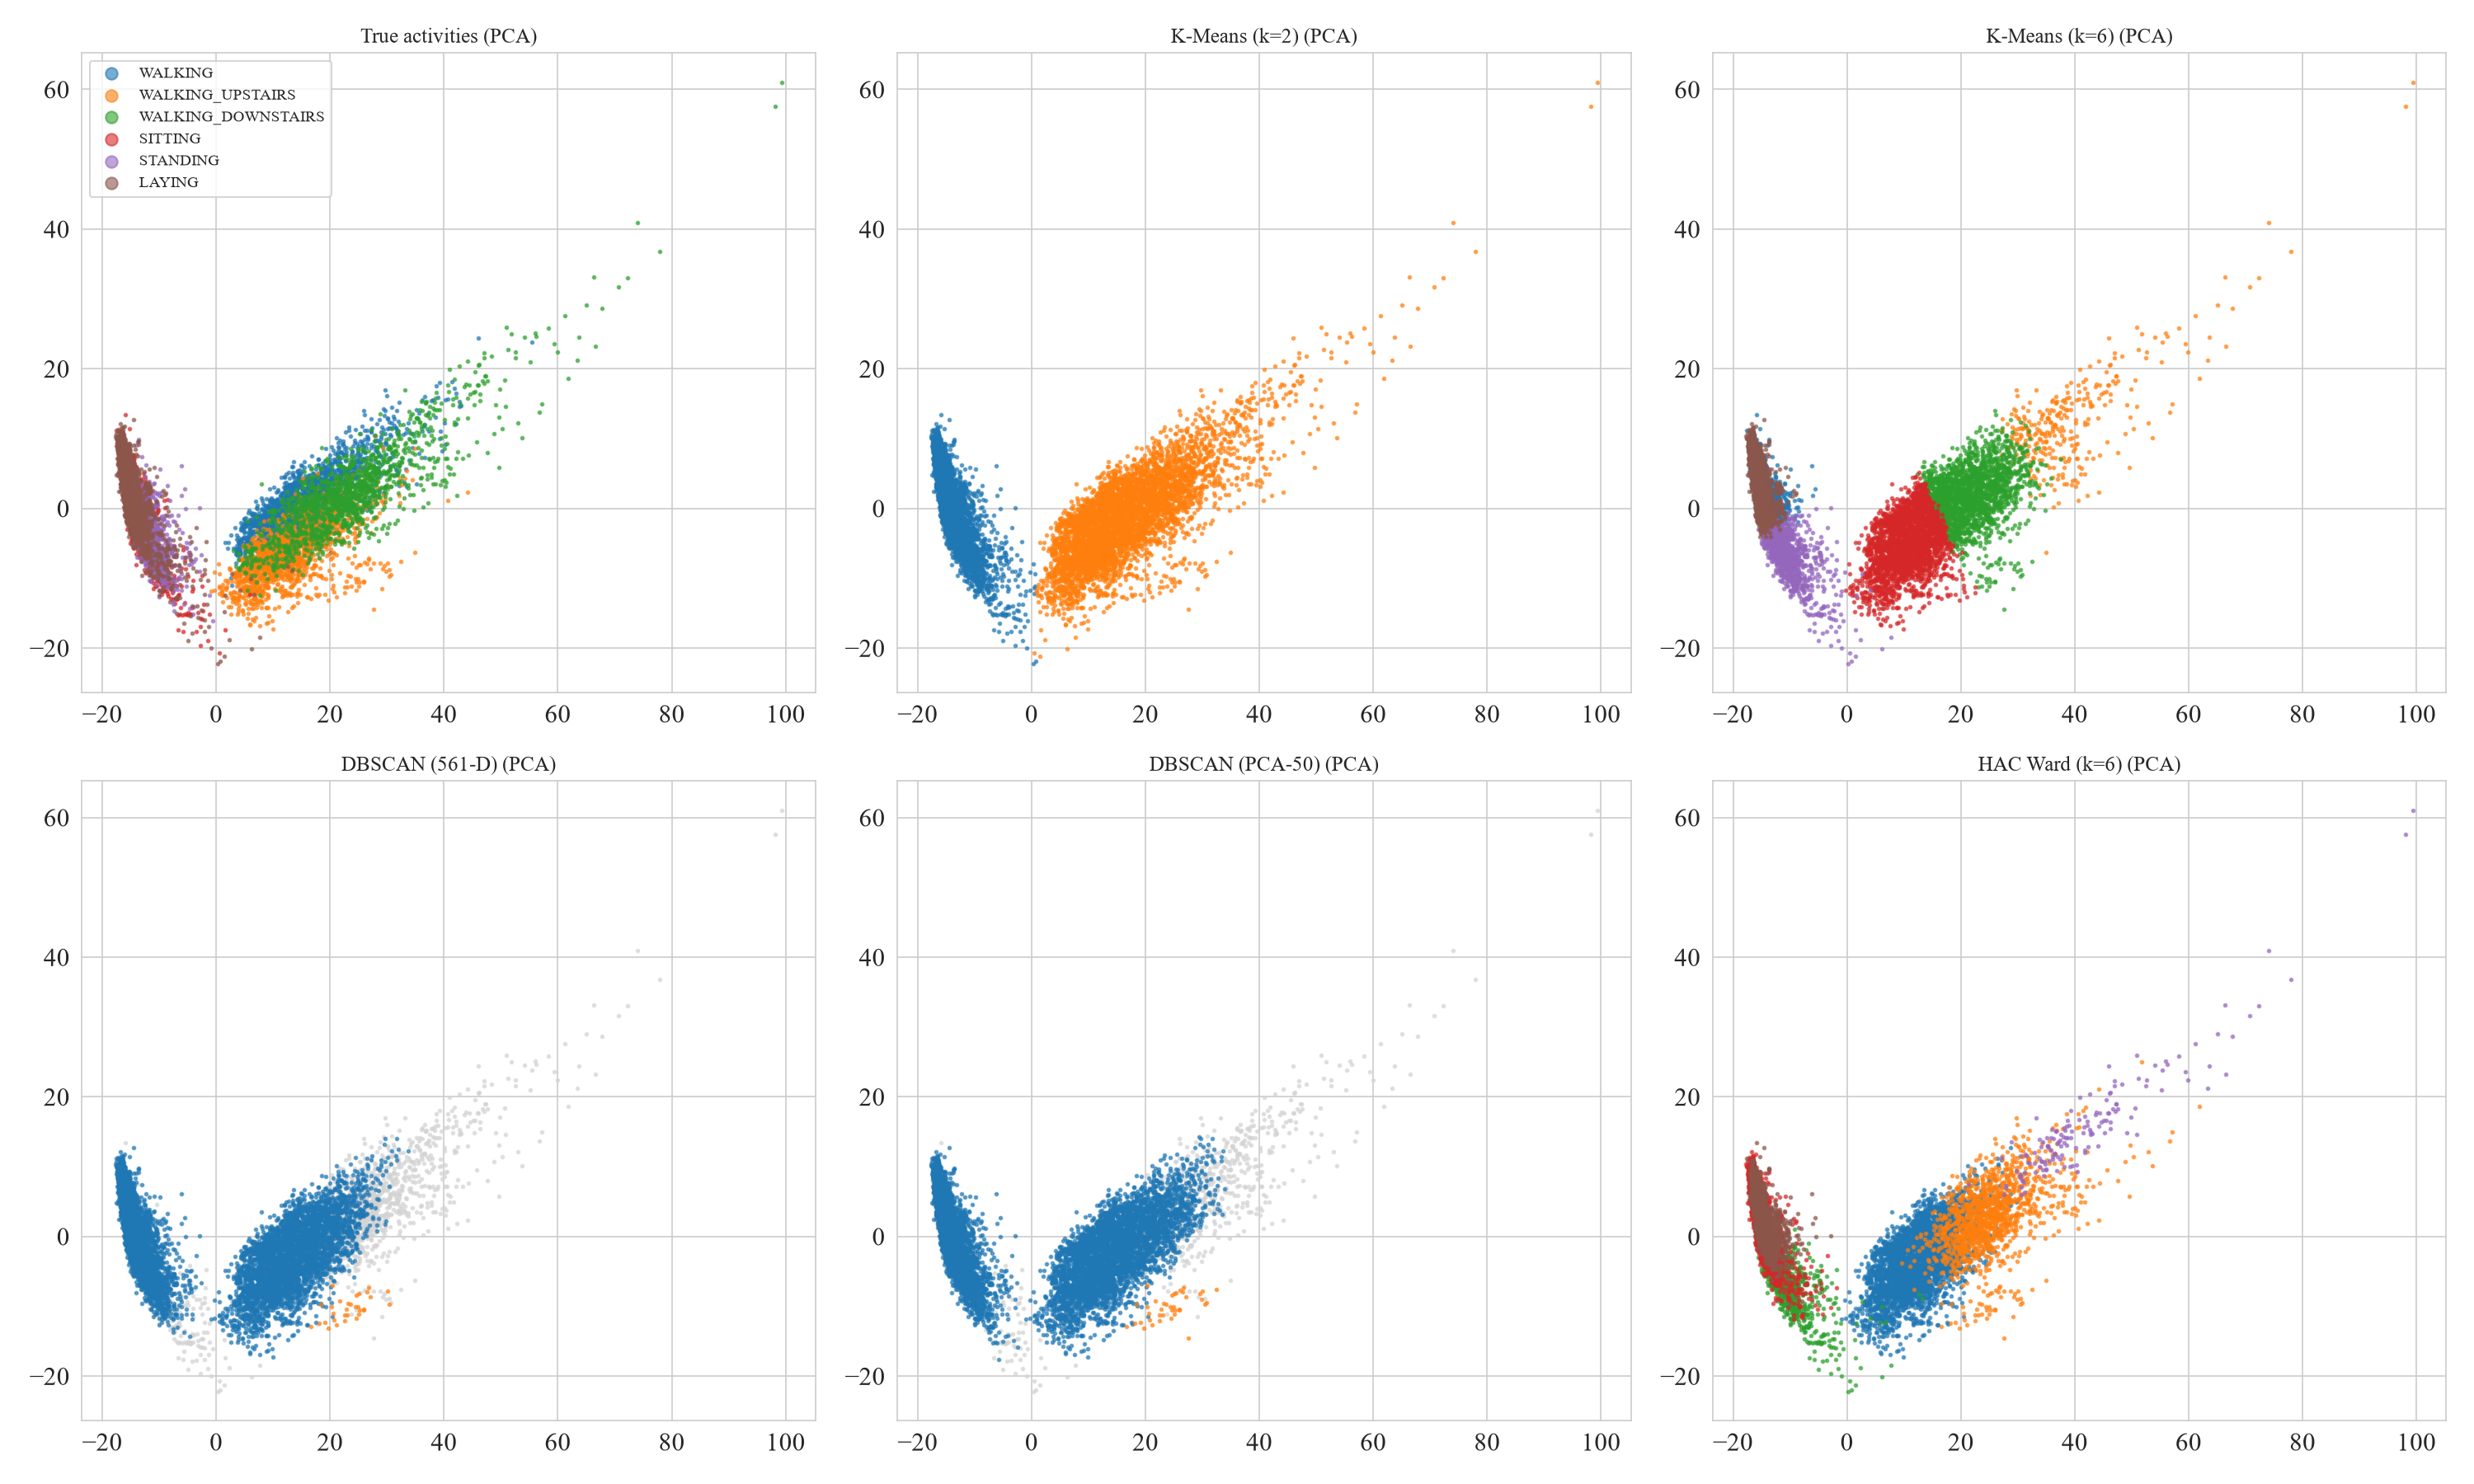
\includegraphics[width=\linewidth]{figures/06_cluster_scatter_pca.png}
\caption{Clusters in the 2-component PCA space. The first panel uses the activity colours of
Figures 1 and 2; in all other panels the cluster colours are arbitrary, and DBSCAN noise is
light grey.}
\end{figure}
\begin{figure}[H]
\centering
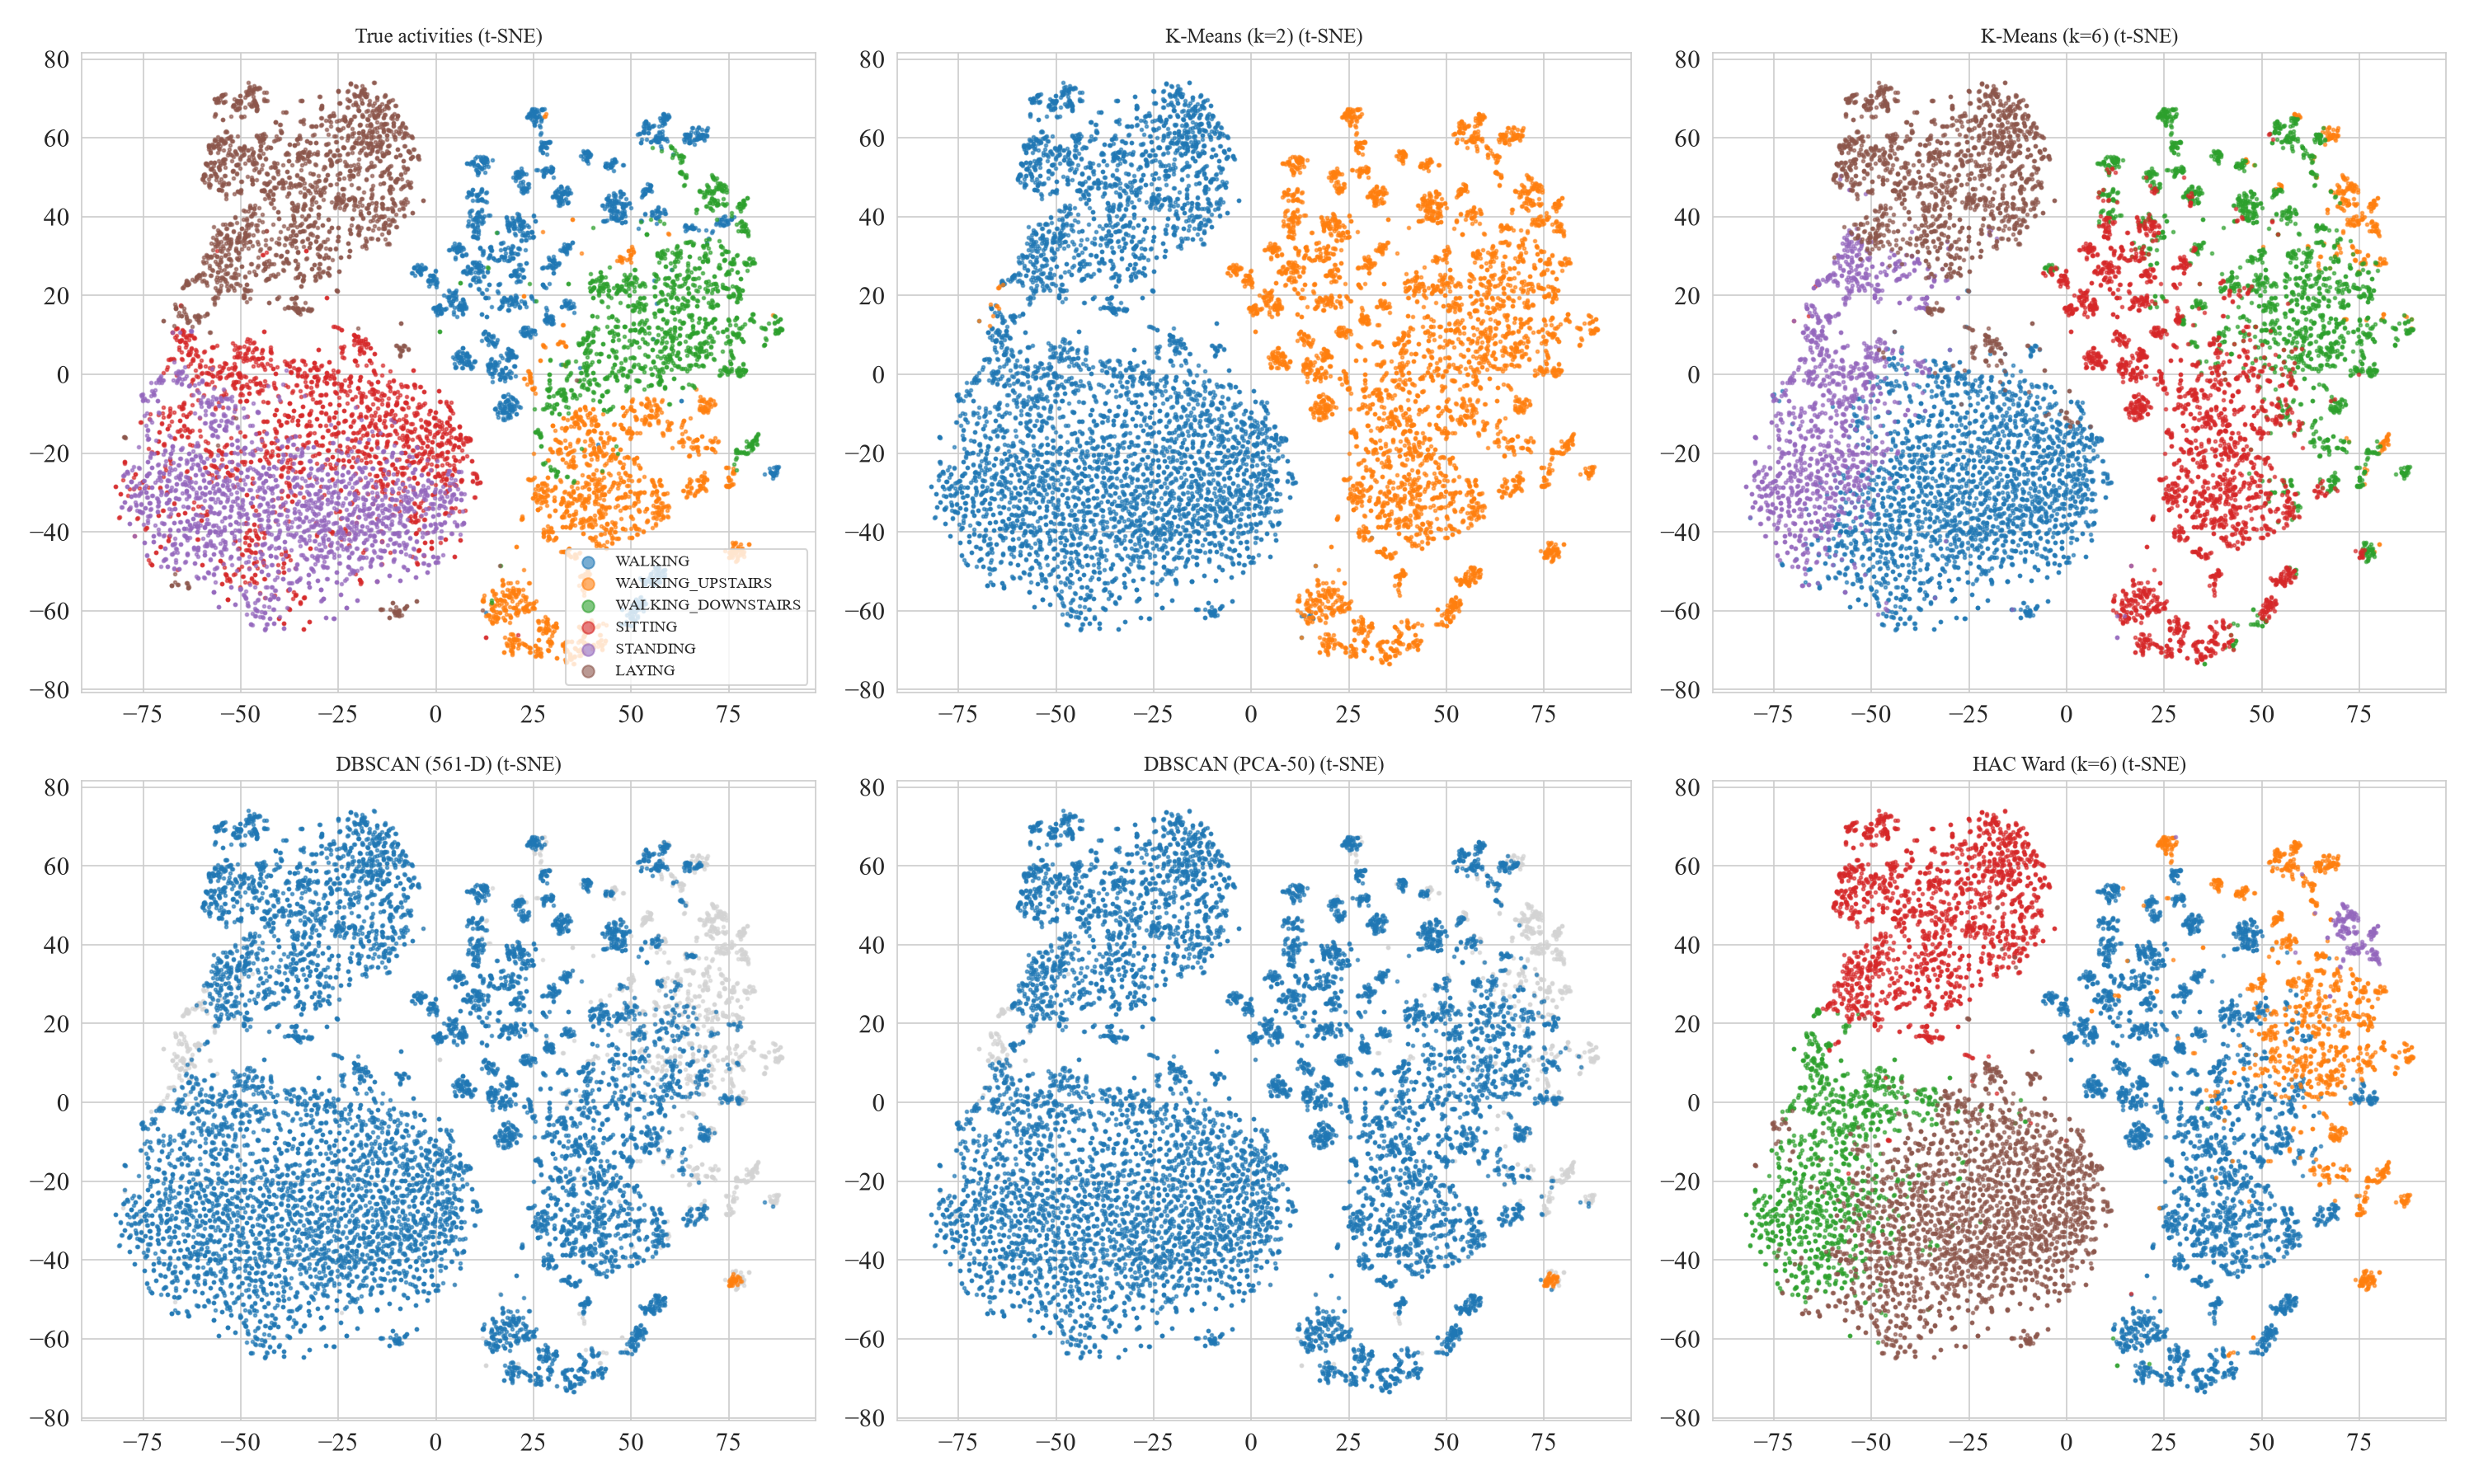
\includegraphics[width=\linewidth]{figures/07_cluster_scatter_tsne.png}
\caption{The same clusterings in the t-SNE space, with the same colour conventions.}
\end{figure}
\textbf{Inference:} K-Means with $k=2$ cuts the PCA cloud between the left static blob and the
right dynamic diagonal. With $k=6$ it slices the dynamic diagonal into bands rather than into
activities, so cluster borders follow distance along the main axis of variation. Both DBSCAN
solutions colour almost everything as one cluster, with the noise points along the upper-right,
sparse end of the dynamic diagonal and around the junction between the two groups, plus a tiny
second cluster. Ward at $k=6$ is
the closest to the true-activity panel, though its clusters still overlap.

\begin{figure}[H]
\centering
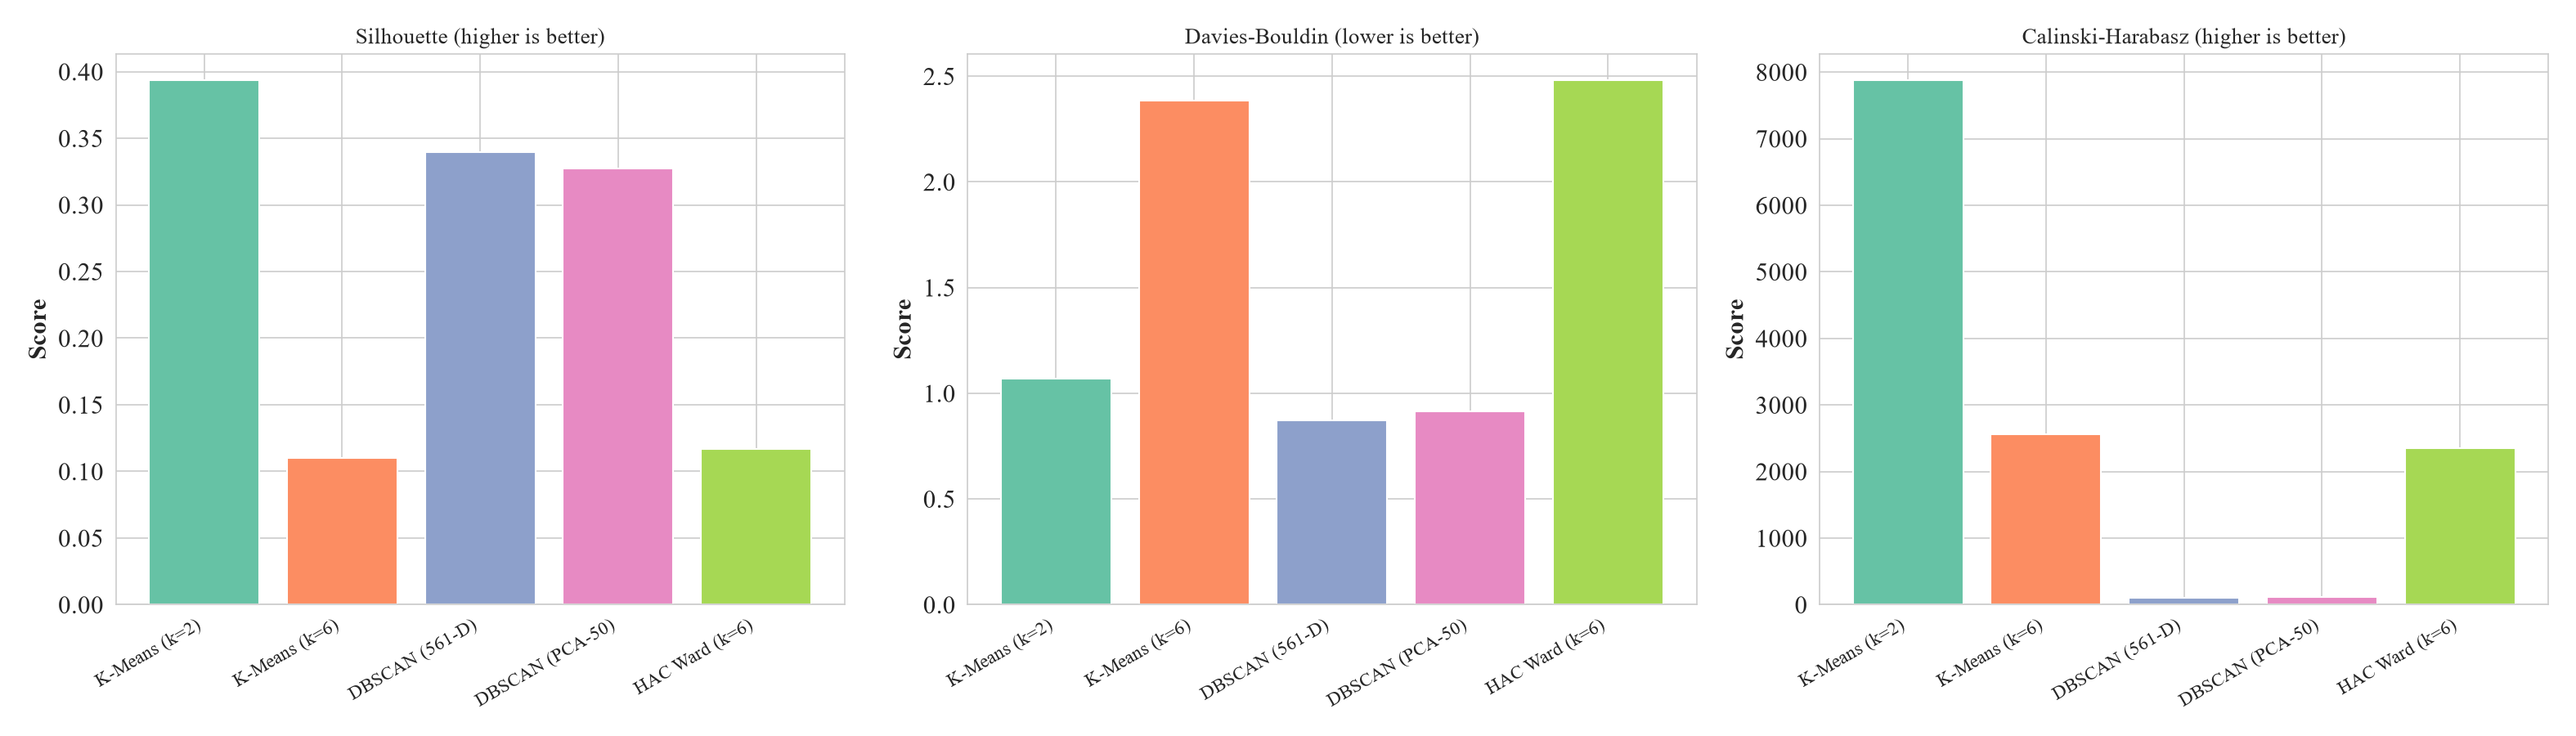
\includegraphics[width=\linewidth]{figures/08_internal_metrics.png}
\caption{Internal metrics (Silhouette, Davies--Bouldin, Calinski--Harabasz) for the five
final clusterings.}
\end{figure}
\begin{figure}[H]
\centering
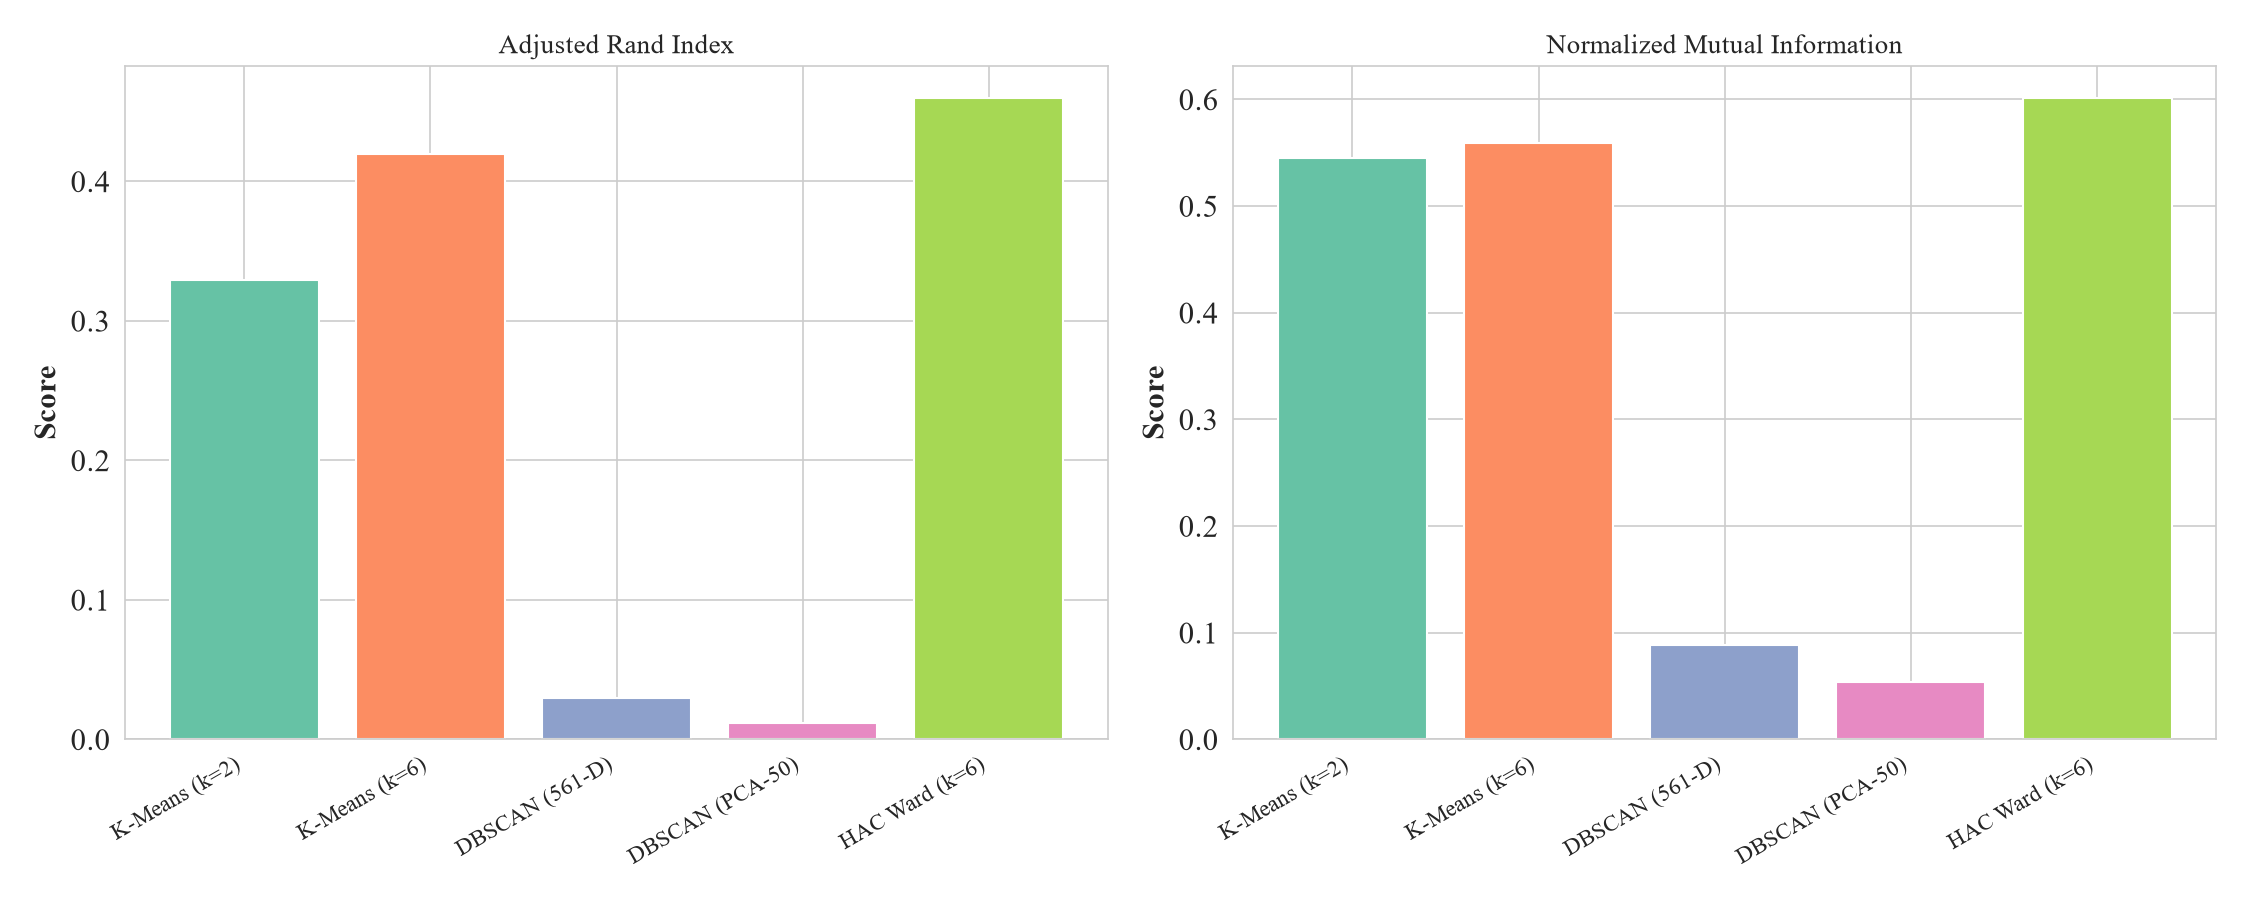
\includegraphics[width=0.85\linewidth]{figures/09_external_metrics.png}
\caption{External metrics (ARI and NMI) against the true activity labels.}
\end{figure}
\textbf{Inference:} The two metric groups rank the models almost in opposite order. K-Means
with $k=2$ and DBSCAN look best on the internal bars, while Ward and K-Means with $k=6$ look best
on the external bars, and both DBSCAN models are near zero on ARI and NMI.

\begin{figure}[H]
\centering
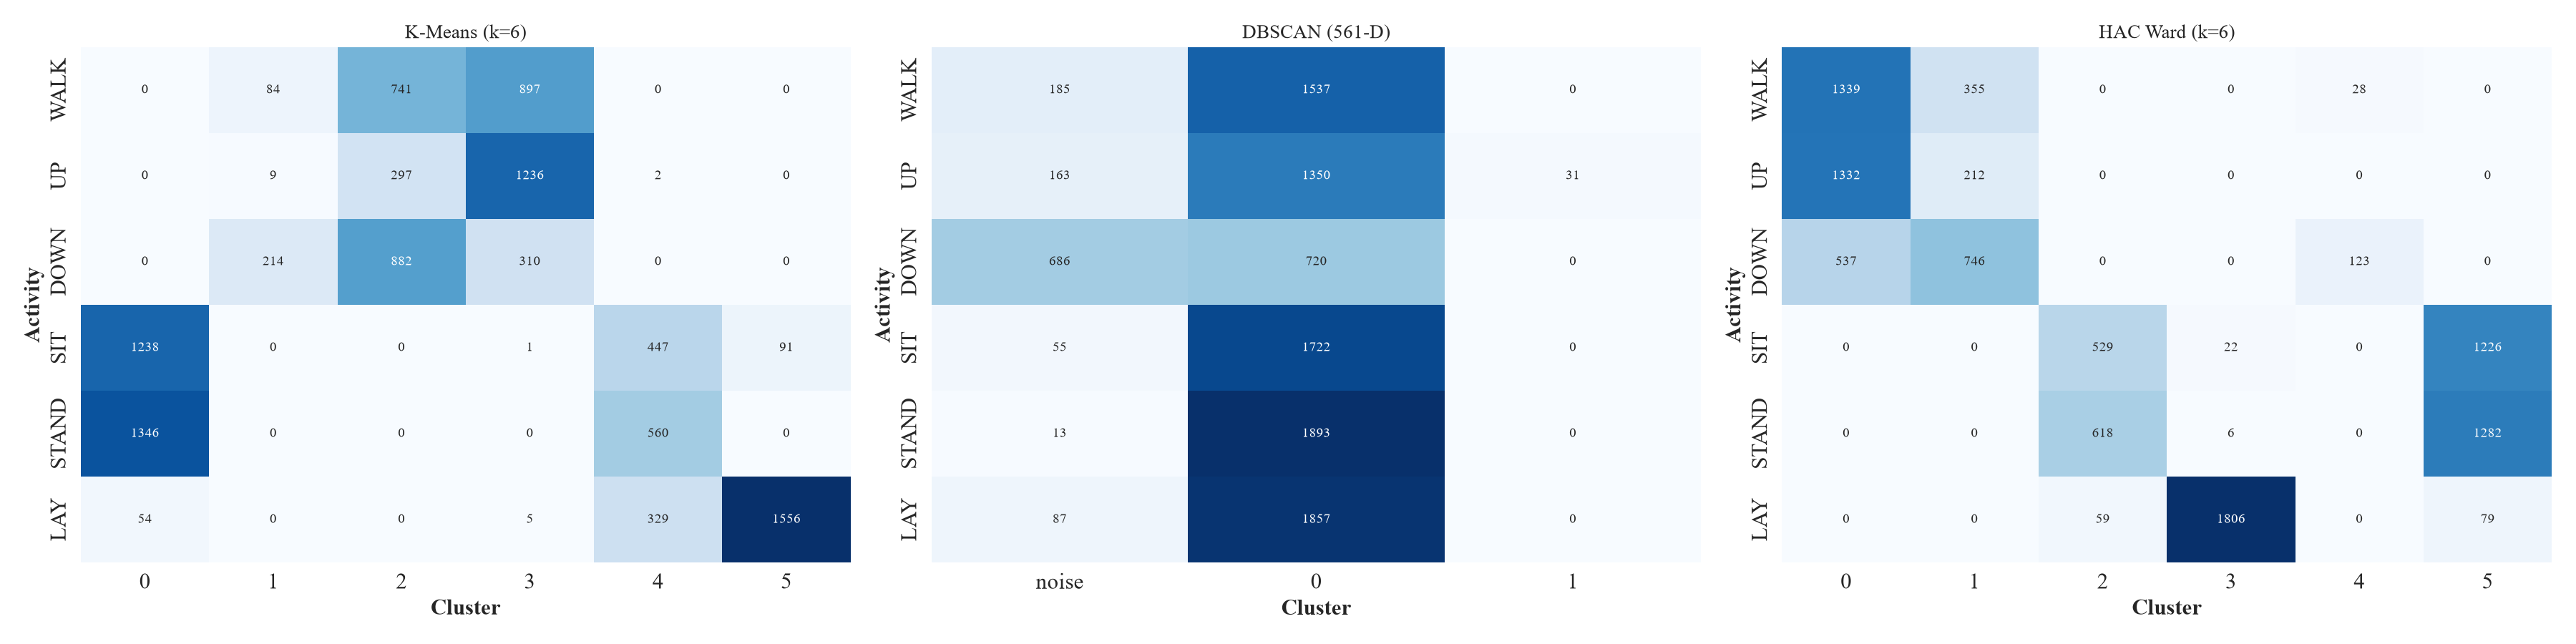
\includegraphics[width=\linewidth]{figures/10_cluster_activity_heatmaps.png}
\caption{Cluster-versus-activity contingency counts for K-Means ($k=6$), DBSCAN (full space)
and Ward ($k=6$).}
\end{figure}
\textbf{Inference:} Laying is recovered well by both six-cluster models (K-Means: 1556 of 1944
in one cluster; Ward: 1806 of 1944 in one cluster). Sitting and standing are never separated;
in both models they are spread almost entirely over the same two clusters. The walking activities are mixed
across two or three clusters each, with walking downstairs the most scattered. DBSCAN puts
nearly every activity in its one large cluster and labels 686 of the 1406 walking-downstairs
windows (49\%) as noise, which is 58\% of all 1189 noise windows.

\section{Discussion}

\subsection*{Observation Questions}
\textbf{1. Which algorithm produced the most meaningful clusters? Why?} It depends on what
``meaningful'' means, and the results show two different answers. Measured against the six
true activities, HAC with Ward linkage is best (ARI 0.4599, NMI 0.6015), just ahead of K-Means
with $k=6$ (0.4196, 0.5593); its largest cluster holds 31.1\% of the windows. Measured by
structure the data actually supports, K-Means with $k=2$ is best: cross-tabulating its two
clusters against the activities shows one cluster holding all of standing (1906), nearly all of
sitting (1774 of 1777) and laying (1932 of 1944), and the other holding all three walking
activities (4664 of 4672), so only 23 of 10,299 windows land on the wrong side of the
static/dynamic divide. DBSCAN was the least meaningful (ARI 0.0298 and 0.0119). None of the
algorithms separated sitting from standing, which look alike to a waist-mounted phone.

\textbf{2. How sensitive was K-Means to the choice of $k$?} Very sensitive. The silhouette
score falls from 0.3937 at $k=2$ to 0.1500 at $k=4$ and 0.0749 at $k=8$; the
Calinski--Harabasz score falls from 7881 to 1975 and the Davies--Bouldin index rises from 1.07 to
2.61, all monotonically or nearly so. The elbow and silhouette rules also disagree (4 versus 2).
ARI is not monotonic in $k$: it stays between 0.29 and 0.33 for $k=2$ to 5, then jumps to
0.4196 at $k=6$ and peaks at 0.4332 at $k=7$. So the internal scores say ``use two clusters''
while the labels say the six-to-seven range recovers the activities better, and the answer
depends on which of the two you trust. The clusters themselves are also unstable in shape:
K-Means slices the dynamic activities by distance along the main axis of variation instead of
following activity boundaries (Figures 6 and 7).

\textbf{3. Did DBSCAN detect noise or small clusters effectively?} Partly. It did isolate a
small, distinct set of atypical windows: at $\epsilon=17.07$, $\texttt{minPts}=10$ it flagged
1189 windows (11.5\%) as noise, and the noise is far from uniform across activities. It covers
686 of 1406 walking-downstairs windows (49\%), against 11\% of walking and of walking-upstairs
windows, 4.5\% of laying, 3.1\% of sitting and 0.7\% of standing. This fits the PCA plot, where the dynamic
activities form the spread-out end of the data. Its only ``small
cluster'' is a 31-window group that consists entirely of walking-upstairs windows. But the
overall result is poor: 9079 windows (88\%) end up in one giant cluster, and no setting in either
grid gave both many clusters and low noise. A single global $\epsilon$ in 561 dimensions does
not fit data whose activities have such different spreads, and the 50-component PCA space did
not fix this.

\textbf{4. How does linkage choice (single/complete/ward) affect hierarchical clustering?}
Enormously. With the tree cut at six clusters, single linkage put 99.9\% of windows in one cluster
(ARI 0.0001), average linkage 98.5\% (ARI 0.0024), complete linkage gave a largest cluster of
54.6\% (ARI 0.3294), and Ward's largest cluster held 31.1\% (ARI 0.4599). Single linkage merges
through the nearest pair of points, so it chains through dense regions and leaves outliers as
singleton clusters; average linkage has the same weakness to a lesser degree. Complete linkage
uses the farthest pair and produces compact clusters but is pulled around by outliers. Ward
minimises the growth in within-cluster variance at each merge, the same criterion as K-Means, which
gives balanced, compact clusters and suits this data. The dendrograms show the same thing:
Ward's tree has one dominant top split, single linkage's is a long chain.

\textbf{5. Which internal metric best matched your visual intuition of cluster quality?}
Calinski--Harabasz. Looking at the scatter plots, the sensible partitions are the two-blob split
and the six-cluster K-Means and Ward solutions, and the bad ones are the single-linkage,
average-linkage and DBSCAN partitions that consist of one giant cluster plus outliers. The
Calinski--Harabasz index ranked exactly those four bad partitions lowest (28.9, 103.2, 120.7 and
161.1) and the four sensible ones highest (7880.8, 2556.5, 2349.7 and 1898.4). Silhouette and
Davies--Bouldin were fooled: silhouette scored single linkage highest of all (0.5601) and average
linkage second (0.4431), and Davies--Bouldin scored single linkage best (0.2733), because a
giant cluster with a few faraway outliers looks well separated. Across the eight
partitions compared (the four linkages, K-Means with $k=2$ and $k=6$, and both DBSCAN models),
the Spearman rank correlation with ARI was $+0.81$ for Calinski--Harabasz, $-0.74$ for
silhouette and $-0.79$ for Davies--Bouldin (a small sample of eight, so indicative, not
conclusive). Calinski--Harabasz also has a bias of its own: it favours compact, roughly
spherical clusters and decreases as $k$ grows, so it can rank models but should not be used
alone to pick $k$; silhouette remained the more useful guide for choosing $k$ within K-Means.

\section{Conclusion}
Clustering 10,299 smartphone-sensor windows with K-Means, DBSCAN and HAC showed that the data
has one strong structure, static versus dynamic activity, which K-Means with $k=2$ recovers almost
perfectly (23 misplaced windows) and which the silhouette, Calinski--Harabasz and
Davies--Bouldin scores all prefer. Recovering the six individual activities is harder. Ward
linkage at six clusters did best (ARI 0.4599, NMI 0.6015), followed by K-Means at $k=6$ (0.4196,
0.5593); both separate laying well but cannot separate sitting from standing and blur the three
walking activities together. DBSCAN, with a single global $\epsilon$, produced one giant cluster,
one tiny second cluster (31 windows in the full space) and 6 to 12\% noise, so it is useful here
mainly as an outlier detector
(it flags half of the walking-downstairs windows). Single and average linkage collapse into one
cluster and should not be used on this data, even though silhouette and Davies--Bouldin rate them
highly; Calinski--Harabasz was the internal metric that agreed best with the true labels.
Limitations: every algorithm was run with one random seed, the DBSCAN grid has only 18 settings per
space, and the hierarchical cut level (6) was fixed by the number of true activities rather than
chosen from the data.

\section{References}
\begin{enumerate}
\item D. Anguita, A. Ghio, L. Oneto, X. Parra, and J. L. Reyes-Ortiz, ``A Public Domain Dataset
for Human Activity Recognition Using Smartphones,'' in \emph{Proc. 21st European Symposium on
Artificial Neural Networks (ESANN)}, Bruges, Belgium, 2013. Dataset available:
\url{https://archive.ics.uci.edu/dataset/240/human+activity+recognition+using+smartphones}
\item M. Ester, H.-P. Kriegel, J. Sander, and X. Xu, ``A Density-Based Algorithm for Discovering
Clusters in Large Spatial Databases with Noise,'' in \emph{Proc. 2nd Int. Conf. on Knowledge
Discovery and Data Mining (KDD)}, 1996, pp. 226--231.
\item L. van der Maaten and G. Hinton, ``Visualizing Data using t-SNE,'' \emph{Journal of Machine
Learning Research}, vol. 9, pp. 2579--2605, 2008.
\item Scikit-learn Developers, ``Clustering,'' Scikit-learn Documentation. [Online]. Available:
\url{https://scikit-learn.org/stable/modules/clustering.html}
\item SciPy Developers, ``Hierarchical clustering (scipy.cluster.hierarchy),'' SciPy
Documentation. [Online]. Available:
\url{https://docs.scipy.org/doc/scipy/reference/cluster.hierarchy.html}
\end{enumerate}

\end{document}
